\documentclass[11pt,a4paper]{scrartcl}
\usepackage[czech]{babel}
\usepackage[utf8]{inputenc}
\usepackage{graphicx}
\usepackage{float}

\begin{document}
	\title{Semestrální práce z předmětu KIV/DS}
	\subtitle{Globální stav v distribuovaném systému}
	\author{Zdeněk Valeš}
	\date{10.1. 2020}
	\maketitle
	\newpage
	
	\section{Zadání}
	Implementace ZeroMQ služby s integrovaným Chandy-Lmportovým algoritmem pro získání konzistentního snímku globálního stavu.
	
	Popis chodu aplikace:
	\begin{itemize}
		\item Implementujte bankovní službu s operacemi (lze využít implementaci z předchozí úlohy) credit a debit tak, že obě operace lze provést na základě zprávy doručené do vstupní ZeroMQ fronty následovně: pokud klient chce poslat částku do jiné banky, odečte částku a pošle zprávu CREDIT s částkou do jiné banky (fronty). Pokud chce klient inkasovat částku z jiné banky, pošle pouze zprávu DEBIT s částkou, přičemž druhá strana částku odečte a pošle ji ve zprávě CREDIT.

		\item Všechny uzly jsou identické, kromě IP adresy a jména uzlu, jejich počet je v rozmezí 2-5
		
		\item Každý uzel po startu začíná se zůstatkem na účtu 5.000.000.

		\item Uzly náhodně vyberou jednu z operací CREDIT či DEBIT s náhodnou částkou v intervalu <10.000, 50.000> a
		odešlou zprávu s operací na náhodně vybraný sousední uzel. Pokud uzel na svém účtu nemá dostatečnou
		částku, operaci odmítne.
		
		\item Uzly spolu komunikují pouze přes vstupní ZeroMQ fronty (podle vzoru PAIR, viz, které představují komunikační kanály. Zprávy
		přenášejte v JSON formátu
		
		\item Topologii si zvolte sami, ale je nutné ji uvést v průvodní dokumentaci
		
		\item Jako servisní službu implementujte Chandy-Lamportův distribuovaný algoritmus pro získání konzistentního snímku globálního stavu podle stejného principu jako bankovní API (zpráva “marker” ve vstupní frontě – viz popis algoritmu)

		\item Spuštění Chandy-Lamportova algoritmu zahajte posláním zprávy MARKER do libovolné fronty (z příkazové
		řádky na libovolném uzlu).

		\item Ošetřete i případ, že může být v jednom okamžiku spuštěno více snapshotů

		\item Stavem uzlu se rozumí zůstatek na účtu v okamžiku přijetí prvního markeru, stavem kanálu seznam zpráv s
		bankovními operacemi přijatými po prvním markeru (viz popis algoritmu)

		\item Jakmile detekujete ukončení algoritmu, všechny uzly pošlou svoje uložené stavy do vyhrazené fronty, ze které
		je vyhrazený proces vybírá a zobrazuje (stačí na konzoli)

		\item K vytvoření infrastruktury použijte nástroje Vagrant a VirtualBox

		\item Aplikaci můžete implementovat v Jazyce Java nebo Python s využitím již existujícího software, který vám
		usnadní implementaci jednotlivých modulů a jejich vzájemnou komunikaci.
	\end{itemize}
	
	
	
	\section{Popis implementace}
	K implementaci jsem si vybral jazyk Python (verze 3). Banky a služba pro sběr globálního stavu spolu navzájem komunikují skrze ZroMQ fronty. Systém obsahuje 4 bankovní servery a jednu službu pro sběr stavu.
	
	\subsection{Topologie systému}
	Topologie systému, společně s IP adresami virtuálních strojů a porty, na kterých služby poslouchají, je znázorněna na obrázku \ref{fig:topology}. Každý virtuální stroj je založen na image \verb|ubuntu/trusty32| -- můj počítač nepodporuje virtualizaci 64 bitových systémů. 
	
	\begin{figure}[H]
		\centering
		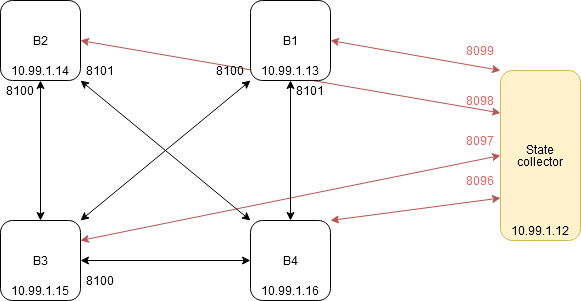
\includegraphics[width=15cm]{img/topologie.png}
		\caption{Topologie systému}
		\label{fig:topology}
	\end{figure}

	\subsection{Konfigurace}
	Bankovní služba při spuštění čte z konfiguračních souborů porty, na kterých má poslouchat a adresy, na které se má připojit. Adresy pro připojení k ostatním bankám a state collectoru jsou ve zvláštních souborech. Příklad csv souboru pro konfiguraci propojení bank:
	
	\begin{verbatim}
1,8100,8101
2,8100,8101
3,8100
4
3,10.99.1.13:8100,10.99.1.14:8100
4,10.99.1.13:8101,10.99.1.14:8101,10.99.1.15:8100
	\end{verbatim}
	
	První sloupec je ID banky, v následujících sloupcích jsou buď porty na kterých banka poslouchá, nebo adresy, kam se připojí.
	
	\subsection{Obecná struktura projektu}
	Zdrojové kódy projektu se nachází ve složce \verb|src|. Bankovní služba je umístěna ve složce \verb|bank|, služba pro sběr globálního stavu je umístěna ve složce \verb|state-collector|. V adresáři \verb|src| je také umístěn \verb|Vagrantfile| obsahující konfiguraci nasazení virtuálních strojů. 
	
	Server je tvořen python skriptem, konfiguračním souborem pro \verb|upstart| a skriptem \verb|bootstrap.sh|, který server inicializuje a spouští. Každý server je na virtuálním stroji veden jako služba. Tím je možné daný server pohodlně vypínat/zapínat. 	Každý ze serverů loguje svou činnost do souboru \verb|log.txt|, skrze který je možné za běhu kontrolovat stav systému. 
	
	\begin{figure}[H]
		\centering
		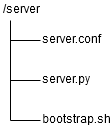
\includegraphics[width=2.5cm]{img/server-structure.png}
		\caption{Obecná struktura složky serveru}
		\label{fig:serv-struct}
	\end{figure}
	
	\subsection{Bank N}
	Každá banka má své unikátní ID. Po spuštění bankovní server přijímá a náhodně generuje zprávy, které posílá svým sousedům. Zprávy jsou odesílány pouze na aktivní sockety (je připojen protějšek). Každý bankovní server má vlastní databázi běžící na daném virtuálním stroji. Struktura zprávy posílané mezi bankami je znázorněna na obrázku \ref{fig:message} -- \verb|type| je \verb|CREDIT|, nebo \verb|DEBIT| a \verb|amount| je částka, se kterou má být daná operace provedena. Speciálním typem je pak zpráva \verb|REFUSE| s částkou nastavenou na -1, která oznamuje neplatnou operaci (na účtu banky není dostatek peněz).
	
	\begin{figure}[H]
		\centering
		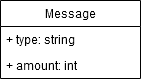
\includegraphics[width=3cm]{img/message.png}
		\caption{Struktura zprávy posílané mezi bankami}
		\label{fig:message}
	\end{figure}
	
	\subsubsection{Připojení k bankovní službě}
	Bankovní služby při připojení provádějí zjednodušený handshake,	aby server (banka, která na socketu poslouchá) mohl rozpoznat, kdy se protějšek připojil. Handshake (znázorněn na obrázku \ref{fig:handshake}) spočívá v odeslání \verb|CONNECTION| zprávy ihned po připojení se k socketu. Po přijetí a potvrzení \verb|CONNECTION| zprávy si server označí daný socket jako připravený a začne na něj odesílat zprávy.

	\begin{figure}[H]
		\centering
		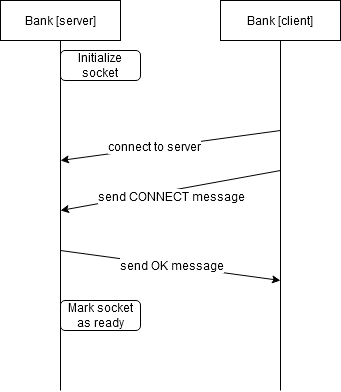
\includegraphics[height=8cm]{img/bank-handshake.png}
		\caption{Handshake mezi bankovními službami}
		\label{fig:handshake}
	\end{figure}
	
	\subsubsection{Chandy-Lamport}
	Součástí smyčky přijmi zprávy/odešli zprávy bankovního serveru je také kontrola, zda se má spustit algoritmus pro detekci globálního stavu. Server pravidelně kontroluje přítomnost souboru pojmenovaného \verb|MARKER| ve svém pracovním adresáři. Pokud tento soubor existuje, server spustí Chandy-Lamportův algoritmus a rozešle zprávy \verb|MARKER| svým sousedům.
	
	Po dokončení algoritmu odešle server svůj zaznamenaný stav a stav komunikačních kanálu state collectoru, který jej zaloguje. 
	
	Aby bylo možné spouštět více snapshotů najednou, obsahuje každá \verb|MARKER| zpráva také unikátní ID, na jehož základě je stav zaznamenán. Jako ID je použito ID banky. Předpokládá se, že jeden uzel nemůže algoritmus spustit vícekrát najednou (musí tedy počkat až jím iniciovaný algoritmus doběhne). Struktura, která v každé bance udržuje lokální stavy (1 stav pro 1 marker id) je znázorněna na obrázku \ref{fig:state-holder}. Výsledný globální stav je pak složen z jednotlivých lokálních stavů všech bank.
	
	\begin{figure}[H]
		\centering
		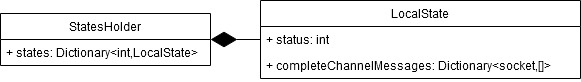
\includegraphics[width=11cm]{img/state-holder.png}
		\caption{Struktura pro udržení lokálních stavů}
		\label{fig:state-holder}
	\end{figure}
	
	\subsection{Služba pro sběr stavů systému}
	State collector po spuštění poslouchá na předem konfigurovaných portech (na které se připojují banky) a vypisuje příchozí zprávy do souboru \verb|log.txt| umístěného v pracovním adresáři.
	
	Výpis stavové zprávy má následující formát:
	
	\begin{verbatim}
		Status message: marker_id=%s; bank_id=%s; status=%s; channel_messages=%s
	\end{verbatim}
	
	Kde \verb|marker_id| je unikátní id použité k rozeznání jednotlivých \verb|MARKER| zpráv. \verb|bank_id| je id banky, která danou stavovou zprávu odeslala, \verb|status| je zůstatek na účtu banky a \verb|channel_messages| jsou zprávy přijaté bankou od odeslání \verb|MARKER| do konce algoritmu.
	
	\section{Spuštění}
	Systém je možné spustit příkazem \verb|vagrant up| v adresáři \verb|src|. Sběr globálního stavu je možné spustit příkazem \verb|touch MARKER| v adresáři \verb|bank| kterékoliv bankovní služby. Globální stav je pak možné přečíst v souboru \verb|state-collector/log.txt| (například příkazem \verb|touch -f state-collector/log.txt|). Příklad výpisu logu, který obsahuje globální stav je na obrázku \ref{fig:global-state}.
	
	\begin{figure}[H]
		\centering
		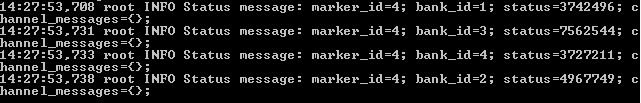
\includegraphics[width=15cm]{img/global-state.png}
		\caption{Příklad výpisu globálního stavu}
		\label{fig:global-state}
	\end{figure}
	
	Poznámka: všechny virtuální stroje mají v konfiguraci vypnutou HW virtualizaci (\verb|["--hwvirtex", "off"]|). V případě, že by to při spuštění dělalo problémy, je možné ji zapnout.
	
	\section{Závěr}
	Práci se mi podařilo úspěšně implementovat. Bohužel, algoritmus je moc rychlý a nepodařilo se mi při testování zachytit stav tak, že by jeho součástí byly neprázdné stavy kanálů.
	
\end{document}
